% Ian Wilkes 
% Artificial Intelligence 600.335
% Assignment 4.
\documentclass[12pt, letterpaper]{article}
\usepackage{amsmath, amsthm, graphicx}


\title{Decision Trees for Classification: \\ An Evolutionary Approach}

\author{Ian Wilkes}

\begin{document}

\maketitle

\begin{abstract}
Classification is one of many extremely important topics within the field of 
artificial intelligence, and is used in many fields from advertising to 
quality control.  As such it is imperative that we be able to provide efficient
and accurate classifiers. One such method for classification is through the use
of decision trees.  This paper will discuss two implementations of decision trees, one using information gain, and another which evolves to learn to classify
sets of data.  Their comparative performance will be discussed, as well as 
ways to optimize each of their individual performance. 


\end{abstract}

\section{Introduction}

\section{Learning Decision Trees}
\subsection{Information-Theoretic Methods}
\subsubsection*{Entropy and Information Gain}
\subsection{Genetic Algorithms}

\subsubsection*{Genetic Algorithms for Decision Trees}

\section{Algorithms and Experimental Methods}

\subsection*{Data Sets}

\section{Results}
\begin{figure}[!htb]
\begin{center}
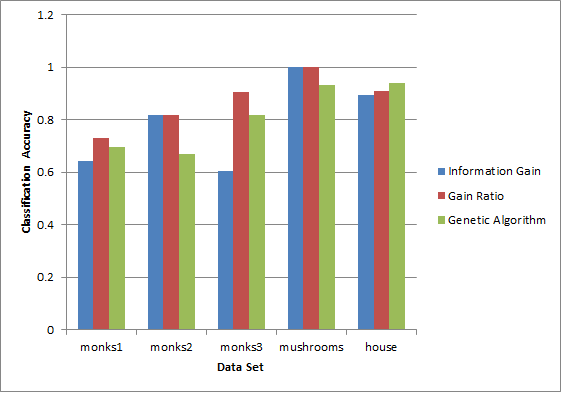
\includegraphics[width=4in]{images/algorithm_comparison_accuracy.png}
\end{center}
\caption{This figure shows the classification accuracy of the information gain
based, gain ratio, and genetic decision trees.  It can be seen that the gain 
ratio based tree seems to perform the best in almost all cases.}
\label{Classification Accuracies of Multiple Decision Trees}
\end{figure}

\begin{figure}[!htb]
\begin{center}
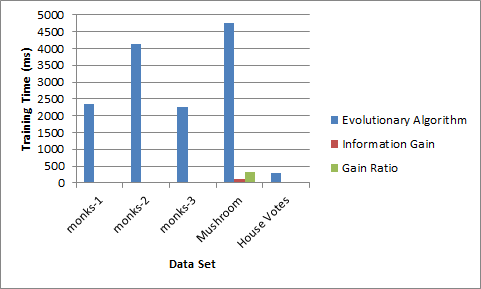
\includegraphics[width=4in]{images/algorithm_comparison_training_time.png}
\end{center}
\caption{This figure shows the required training times of the information gain
based, gain ratio, and genetic decision trees.  It can be seen that the genetic
tree takes much more time than either of the other trees.}
\label{Training Times of Multiple Decision Trees}
\end{figure}

\begin{figure}[!htb]
\begin{center}
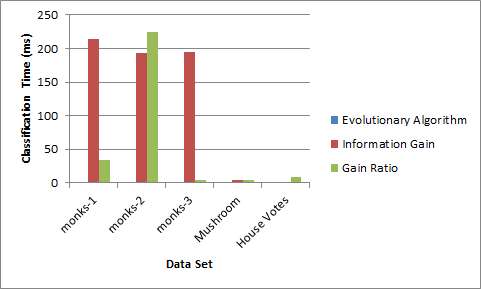
\includegraphics[width=4in]{images/algorithm_comparison_testing_time.png}
\end{center}
\caption{This figure shows the testing time of the information gain
based, gain ratio, and genetic decision trees.  Here, the evolutionary or 
genetic tree takes orders of magnitude less time than the information based
trees.}
\label{Testing Times of Multiple Decision Trees}
\end{figure}


\begin{figure}[!htb]
\begin{center}
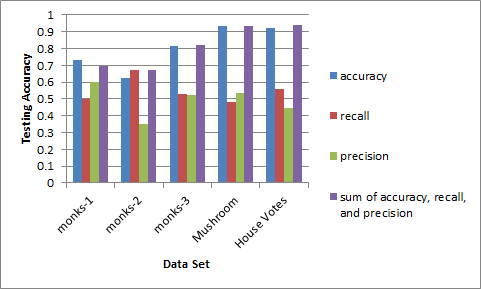
\includegraphics[width=4in]{images/fitness_comparison.png}
\end{center}
\caption{This figure shows the results of using different fitness functions on
the classification accuracy of the genetic tree.}
\label{Classification Accuracies Using Various Fitness Functions}
\end{figure}


\begin{figure}[!htb]
\begin{center}
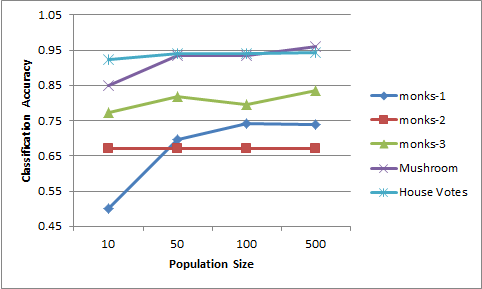
\includegraphics[width=4in]{images/population_comparison.png}
\end{center}
\caption{Here the performance of the genetic algorithm on different data sets
is shown for different population sizes.  For four of the five data sets, the
population must be above 10 individuals to get the best classification accuracy.
}
\label{Testing Times of Multiple Decision Trees}
\end{figure}



\begin{figure}[!htb]
\begin{center}
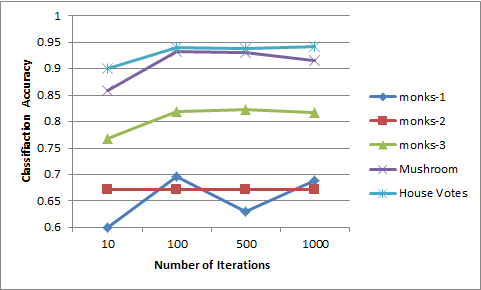
\includegraphics[width=4in]{images/iteration_comparison.png}
\end{center}
\caption{Here the performance of the genetic algorithm on different data sets
is shown for different numbers of training iterations.  For four of the five 
data sets, at least 100 iterations are required to get optimal classification 
accuracies.  
}
\label{Testing Times of Multiple Decision Trees}
\end{figure}

%7
\begin{figure}[!htb]
\begin{center}
\includegraphics[width=4in]{images/mutation_comaprison.png}
\end{center}
\caption{This plot shows the effects of different mutation probabilities on
the classification accuracy of the genetic algorithm for different data sets.  
From this data, it seems that whether or not mutation is beneficial depends on
the particular data set, with an increase helping in some cases, and hurting
in others.
}
\label{Testing Times of Multiple Decision Trees}
\end{figure}

%8
\begin{figure}[!htb]
\begin{center}
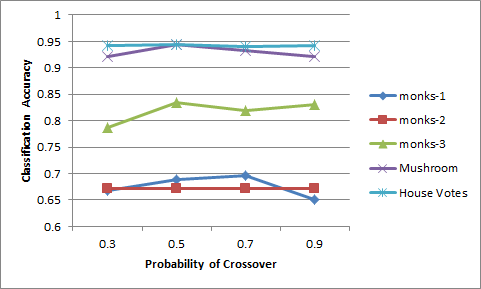
\includegraphics[width=4in]{images/crossover.png}
\end{center}
\caption{The above figure of the effects of different crossover probabilities on
classification performance shows a similar trend to that of the mutation plot,
with some data sets benefiting from increased crossover, while others are hurt.
}
\label{Testing Times of Multiple Decision Trees}
\end{figure}


%9
\begin{figure}[!htb]
\begin{center}
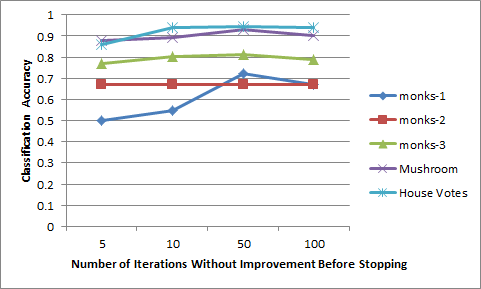
\includegraphics[width=4in]{images/cutoff_accuracy.png}
\end{center}
\caption{This plot shows the effects of the cutoff value on the classification
accuracy of the genetic algorithm for different data sets.  The accuracy seems
to plateau after a certain cutoff value, indicating little effect.
}
\label{Testing Times of Multiple Decision Trees}
\end{figure}

%10
\begin{figure}[!htb]
\begin{center}
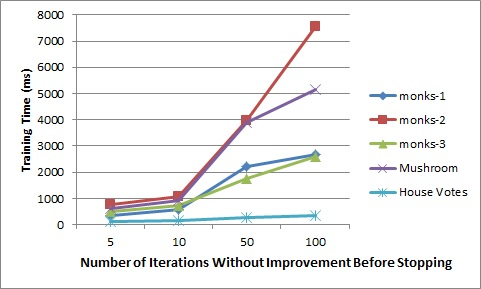
\includegraphics[width=4in]{images/cutoff_time.jpg}
\end{center}
\caption{It can clearly be seen that the time required for training to finish
increases drastically as the cutoff parameter increases for all data sets. 
}
\label{Testing Times of Multiple Decision Trees}
\end{figure}

\begin{table}
\begin{center}
\begin{tabular}{|c||c|cc}
\hline
& col1 & col2 & col3\\
\hline \hline
row1 & a & b & c\\
\hline 
row2 & d & e & f\\
\hline 
row3 & g &   & h\\
 & i & j & k\\
\hline 
\end{tabular}
\end{center}
\caption{This is a caption on the table.  Try to keep your captions short; don't
put multiple paragraphs of text in here.  Put the long version in the Results
section, and reference the table from there.}
\label{sometable}
\end{table}

For all the data shown in this section, the basline genetic algorithm used the 
following parameters which were determined through minimal testing by hand.  
All parameters remain constant, except in the case where they are being
examined one by one.  The mutation and crossover probabilities were 0.01 and 
0.7 respectively.  The population size was 50, and 100 iterations were 
performed.  The default cutoff value was 50.
The standard fitness function used was the sum of the classification accuracy,
recall and precision for each iteration.  Finally, all data presented here is 
the average of five trials for each data point.  

From figure 1 we can see that the performances of the genetic, information
gain and gain ratio based trees are all somewhat comparable.  The gain ratio
tree seems to perform the best of the three in all but the house votes data set.
It drastically out performs the information gain based tree on the monks-3 data
set, whcih is also beaten by the genetic algorithm.

Moving on to figure 2, it is plain to see that the evolutionary algorithm
takes much longer to train than the traditional decision trees, neither of which
ever takes even 500ms to train, while the genetic tree takes almost 5000ms on 
the mushroom data set.

The opposite trend can be seen in the classification times of the testing sets,
which can be observed in figure 3.
The information gain and gain ratio trees take orders of magnitued more time
to classify their data on the monks-1, monks-2, and monks-3 data sets than the
genetic tree.

Figures 4 through 10 show the results from various experiments performed to 
try to optimize the genetic tree shown above. The first of these is figure 4
which shows the effect on classification accuracy of various fitness functions.
It can clearly be seen that by not using the accuracy as one of the components
of the fitness function, the resulting classification accuracy is greatly
reduced, as seen in the cases where recall and precision were used as the 
fitness metrics.

Another parameter which was varied was the population size within the genetic
algorithm based tree.  From figure 5, it can be seen that below a certain 
population threshold the classification performance decreases, yet above that
threshold, an increase in population size does not neccesarily result in 
improved classification performance. The same trend can be seen for the number
of iterations used to train the tree in figure 6. Other than the monks-2 data 
set, all data sets showed a classification accuracy increase by increasing the
number of iterations from 10 to 100.

The effects of mutation and crossover probabilities can be seen in figures 7 
and 8 respectively.  In both cases, the change in the probabilities seem to 
cause different results for the different data sets.  Increasing the mutation
seems to hurt the Mushroom accuracy, while it helps the monks-1 accuracy going
from 0.03 to 0.05.  Similarly for crossover, accuracy is highest for monks-3 
when the crossover probability is 0.9, but this value causes the accuracy for
both the monks-1 and mushroom data sets to decresse significantly.  

Finally, the influence of the cutoff parameter, which stops iteration if no
improvements have been found after a given number of iterations, is shown in
figures 9 and 10. In figure 9, the effect on accuracy can be seen to be minimal
for high values of the cutoff parameter, as the performance for most data sets
stays fairly constant. Figure 10 shows that while the performance may not 
change, the computation time to train the GA increases substantially.    


\section{Discussion}
\subsection{Algorithm Comparison}
From the results shown above, it can be seen that the genetic algorithm does not
perform as well as the gain ratio decision tree.  This tree almost across the
board produced the best classificatio accuracies.  It is always equal to or
better than the information gain tree, as it uses that same information gain,
but can also determine which variables can acutally produce strong results 
outside of the training set. This is a pitfall of the information gain tree
which is particularly apparent on the monks-3 data set, where unique IDs are 
provided for all cases.  Here the information gain tree picks that attribute
as having by far the most information gain, without reallizing that this will
overfit the data.  By instead using the gain ratio, this problem is overcome, 
and an accuracy of approximately 90 percent is achieved on the very same data
set by the gain ratio tree. The tradeoff however is really seen by looking at
the testing and training time graphs. While the genetic tree takes significantly
longer to train than the decision based models due to maintaining many trees and
iterating on them many times to produce useful trees, its classification time
is significantly smaller, presumably due to it creating smaller trees than the
traditional algorithms.  The other possibility for this result would be that 
the genetic tree was implemented more efficiently than the traditional trees,
which is certainly a possibility, but seems unlikely.  It is unlikely, because
their classification times are significantly different on the monks-1 and 
monks-3 data sets while they both are implemented on almost exactly the same
manner.  
\subsection{Genetic Algorithm Parameters}

Moving now to the effects of the various parameters of the genetic algorithm,
it is as expected that the fitness function would have an extreme impact on
the resulting classification accuracy, as with recall and precision, both
false positives and negatives are not minimzied at the same time.  As such,
only the cases where the accuracy was a part of the fitness function produced
good results.  Perhaps the one exception to this is the monks-2 data set, where
the recall fitness function performed equally well if not better than the sum
and accuracy fitness functions.  

Moving on to the population and iteration experiments, it is somewhat surprising
that the performance does not improve with additional members or iterations.  
It is also shocking that increasing either would decrease the accuracy, as 
can be seen by using 500 iterations on the monks-1 data set.  This and other
similar artifacts are probably due to the random nature of the genetic algorithm
where in some cases, a very good individual is randomly created, so even
the smaller population and iteration cases could have produced very high
classification accuracies.  This could be partially resolved by running more
trials to reduce the standard deviation from the expected value, which would
presumably not have the same wavering charateristics.  It is also expected that
if too few iterations are used, or too few members of a population are used, 
that the performance will be poor, as each additional member allows for another
random chance to get a good individual which will then be used to do the final
classification.  For minimal iterations, there is not time to spread good
traits to other members to optimize the resulting tree, and thus the same 
behavior is expected. 

Perhaps the most unexpected of all the trends is that neither the mutation rate
or the crossover rate seem to have a strong effect on the classification
accuracy.  This would seem to imply that the swapping of parts of the trees or
changing random parameters had little effect on the resulting classifications, 
indicating that it is simply the luck of the draw for good random trees at the
first stage of the process which produces the best results.  This result is
somewhat similar to that from the experiments with the population size and
number of iterations, which both seem to plateau the performance after a 
given number.  If crossover and mutation have little effect on the performance
of a tree, then by iterating many times, there will be few changes, and as a
result more iterations will not provide better classification results.

Again the same trend can be seen in the cutoff data, as after the cutoff gets
to a certain point, increasing it no longer has an effect on the performance.  
Again, if the crossover and mutation do not result in improvements in 
classification performance, then even given more iterations to improve,
it is unlikely that the best tree will change, so higher cutoffs have little
effect, other than to drastically increase the time required to train the set. 
This also shows us that these algorithms are simply cutting off early, instead 
of producing better trees with more iterations, either due to convergence, or
the lack of effects from mutation and crossover.



\section{Conclusions}
% many different styles of bibliography are available; plain is fine for this
% assignment
\bibliographystyle{plain}

% the bibliography command should contain the name of your .bib file, minus the
% extension.
\bibliography{templateBibliography}

% because "document" is an environment, you need to have a closing tag at the
% end of your document.  Anything written after this tag will not be included in
% the generated output.
\end{document}
